\documentclass[a4paper]{article}

%------------------------------------------------------------
% PACKAGES
% Base Packages
\usepackage[ngerman]{babel}
\usepackage[utf8]{inputenc}
\usepackage[T1]{fontenc}
\usepackage{geometry}
\usepackage{subfiles}
\usepackage{xcolor}
\usepackage{graphicx}
\usepackage{pdfpages}
\usepackage{todonotes}
\usepackage{listings}
\usepackage[backend=bibtex, style=ieee, citestyle=ieee]{biblatex}
\usepackage{csquotes}

% Misc Packages
\usepackage{svg}
\usepackage{fancyhdr}
\usepackage{authblk}

% End Packages
%------------------------------------------------------------

%------------------------------------------------------------
% DEFINITIONS
% Color Definitions
\definecolor{codegreen}{rgb}{0,0.6,0}
\definecolor{codegray}{rgb}{0.5,0.5,0.5}
\definecolor{codepurple}{rgb}{0.58,0,0.82}
\definecolor{backcolour}{rgb}{0.921, 0.929, 0.937}

% Listings Definitions
\lstdefinestyle{mystyle}{
	backgroundcolor=\color{backcolour},   
	commentstyle=\color{codegreen},
	keywordstyle=\color{magenta},
	numberstyle=\tiny\color{codegray},
	stringstyle=\color{codepurple},
	basicstyle=\ttfamily\footnotesize,
	breakatwhitespace=false,         
	breaklines=true,                 
	captionpos=b,                    
	keepspaces=true,                 
	numbers=left,                    
	numbersep=5pt,                  
	showspaces=false,                
	showstringspaces=false,
	showtabs=false,                  
	tabsize=2
}
\lstset{style=mystyle}
%------------------------------------------------------------


%------------------------------------------------------------
% SETTINGS
% Bibliography settings
%\addbibresource{example.bib} % Add your own bibtex file here

% Geometry / Margin Settings
\geometry{
	paper=a4paper, % Change to letterpaper for US letter
	inner=2.5cm, % Inner margin
	outer=3.8cm, % Outer margin
	bindingoffset=.5cm, % Binding offset
	top=1.5cm, % Top margin
	bottom=1.5cm, % Bottom margin
	%showframe, % Uncomment to show how the type block is set on the page
}

% Paths
\graphicspath{{images/}}
\svgpath{{images/svg/}}
\pagestyle{fancy}
\fancyhf{}

% End Geometry / Margin Settings
%------------------------------------------------------------

%------------------------------------------------------------
% DOCUMENT SPECIFIC
% Author
\author{
	Deniz Akca
	\and
	Dennis Bannerman
	\and
	Mike Iten
}
\affil{ZHAW - Zurich}

% Project
\newcommand{\project}{Projektarbeit Aquaponik}
\newcommand{\outline}{Anforderungsanalyse und Umsetzung einer Software-Lösung im Bereich Aquaponik am Beispiel der ZHAW Wädenswil}

% Title
\title{
	\Huge{}\color{blue}\textbf{\project}\\ 
	\vspace{2cm}
	\large{}\color{black}\textbf{\outline}
}

% Define titlepage layout
\makeatletter
\def\@maketitle{%
	\newpage
	\null
	\vskip 1cm%
	\begin{center}%
		\let \footnote \thanks
		{\LARGE \@title \par}%
		\vskip 2cm%
		{\large
			\lineskip .25em%
			\begin{tabular}[t]{c}%
				\@author
			\end{tabular}\par}%
		\vfill%
		{\large \@date}
	\end{center}%
	\par
	\vskip 1.5em
}
\makeatother

%------------------------------------------------------------

\begin{document}
	\sloppy
	\pagenumbering{roman}
	
	\begin{titlepage}
		\maketitle
		\thispagestyle{empty}
	\end{titlepage}
	
	\tableofcontents
	\newpage
	
	% Page numbering is arabic henceforth
	\pagenumbering{arabic}
	\fussy
	

		
	\section{Einleitung}
	
	\subsection{Ausgangslage}
	Ein Aquaponics Projekt besteht bereits aus folgenden Komponenten. Sensoren der Aquaponics Systeme, welche an SC1000 Geräten angeschlossen sind. 
	Ein serieller Bus verknüpft alle SC1000 mit einem RasPi welches über eine Modbus-API die Sensordaten auf eine MySQL Datenbank ablegt. Diese Daten werden auf der Webseite dargestellt.
	

	Die Webseite, welche unter myaquaculturefarm.ch zu finden ist, wird auf hosttech.ch gehostet. Hosttech verwendet als Backend Technologie PHP.
	Unsere Konfigurationsseite wird ebenfalls auf dieser Domain parallel zu den anderen Webseiten von ZHAW Life Sciences und Facility Management gehostet.
	
	Beim Backend sind wir gebunden was die Host-Firma uns zur Verfügung stellt, in diesem Falle wäre das PHP.
	
	\subsection{Aufgabenstellung}
	Die Datenbank, in der die Sensordaten geloggt werden, besteht aus zwei Tabellen. In einer der Tabellen werden die Sensoren eingetragen, die sich in den Systemen befinden und in der zweiten Tabelle werden die Sensordaten abgespeichert und mit dem jeweiligen Sensor verknüpft.
	
	Das Bearbeiten dieser Zuordnungstabelle ist für die Mitarbeiter/Studierende der ZHAW Life Sciences und Facility Management mit dem von Hosttech gegebenen Tool «phpMyAdmin» nicht verständlich. Zusätzlich müssen spezifische Werte eingegeben werden die einen Informatik Laien nicht bekannt sind, welches zu inkorrekte Angabe von Daten führen kann, welches wiederum zu einem Durcheinander in der Log-Tabelle führt. 
	Das «phpMyAdmin» Tool ist ebenfalls nur per Verwaltungsseite der Hosttech Domain erreichbar welches eine zusätzliche Hürde darstellt.
	
	\subsection{Zielsetzung}
	Um die Zuordnuntabelle einfacher zu bearbeiten, soll der Ablauf abgändert werden. Als Lösung stellen wir eine REST Schnittstelle zur Verfügung über welche die Tabelle mit wenigen Handgriffen verändert werden kann. 
	Diese soll übersichtlich und einfach zu bedienen sein. Damit die Schnittstelle zu jeder Zeit erreichbar ist soll sie gehostet werden.
	
	\section{Grundlagen}
	
	\subsection{Hosting}
	Wir sind nicht zufrieden mit Hosttech und möchten gerne ein anderes Backend als PHP einsetzen, daher haben wir uns entschieden die Verwaltungswebseite auf einem anderen Anbieter zu hosten. 
	Hierbei hat unser Betreuer seine Plattform angeboten. Auf dieser können wir ein Image des Dockercontainers hosten lassen. Somit ist dieses zu jederzeit erreichbar. Dies gilt für das Frontend sowie für das Backend.
	Damit der Server nach der Umsetzung nach wie vor erreichbar ist, wurde uns vom Betreuer folgende Seite vorgeschlagen: https://www.hetzner.com/de/
	
	\subsection{Backend Technologie}
	Mit dem Loslösen von Hosttech sind wir frei die Backend Technologie zu bestimmen und wir haben uns auf Java/Spring geeinigt. Wir haben uns für Spring entschieden, da alle Entwickler mit Java vertraut sind und OpenAPI Spring unterstützt. 
	
	\subsection{Schnittstelle}
	Als Schnittstelle zwischen Backend und Frontend wollen wir das State of the Art Tool OpenAPI einsetzen. Nach genauerer Analyse sehen wir einen grossen Nutzen des Tools, da es uns eine grosse Unterstützung zur Entwicklung der REST Schnittstelle sein wird. 
	
	\subsection{Frontend Technologie}
	Als Frontend-Framework sind wir frei, da es keinen Wunsch/Voraussetzung vom Kunden gab.
	Wir als Gruppe haben uns für Angular(2+) entschieden, da die Mehrheit der Gruppe sich mit diesem Framework gut auskennt. 
	
	\subsection{Datenbank}
	Um den alten Stand weiterzuführen, wird weiterhin die mySQL Datenbank benutzt. Diese wird mithilfe der Schnittstelle angepasst.
	
	\section{Vorgehen / Methoden}
	
	\subsection{Swagger}
	Erste Umsetzungen finden mithilfe eines Swaggerprojekts statt. Hier kann ein Entwurf erstellt werden. Mithilfe dieses Entwurfs wird ein Grundgerüst hergestellt, welcher dazu dient, vereinfacht die REST Schnittstelle zu bauen.

	\begin{figure}[h]
		\centering
		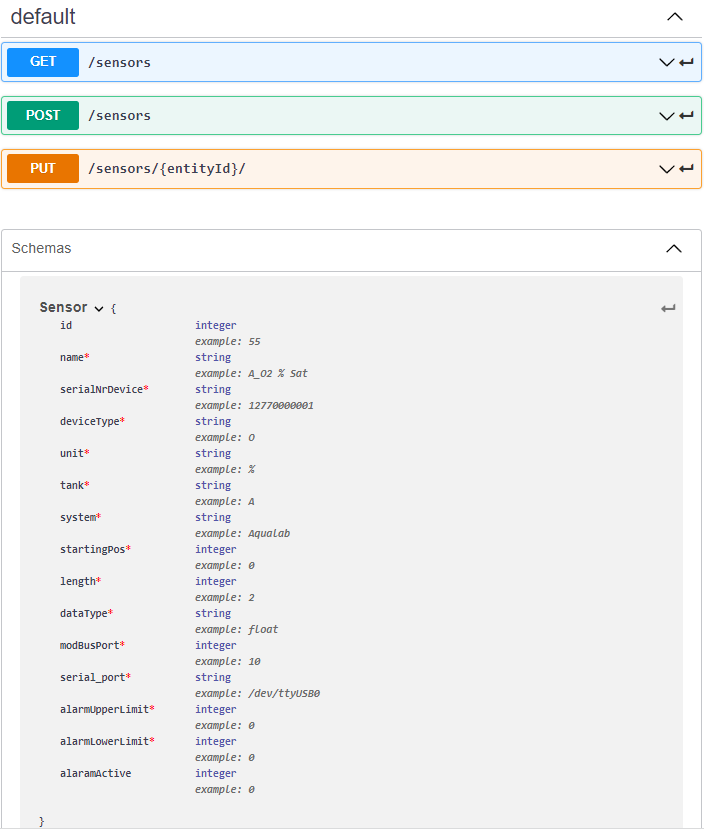
\includegraphics[scale=0.4]{Swagger}
		\caption{Swagger Beispiel}
		\label{fig:Swagger}
	\end{figure}

	Die Schnittstelle soll dazu fähig sein Daten der Sensoren zurückzugeben. Die Möglichkeit soll bestehen, dass die Sensorendaten zusätzlich editierbar sind.
	
	Als Vereinfachung können die Sensoren auch als eine Liste angezeigt werden.
	
	\subsection{Docker}
	
	
	\section{Resultate}
	\section{Diskussion und Ausblick}
	
	\subsection{Sprint 0 Meeting}
	\begin{itemize}
		\item Angular Demo von  Herr Bachmann TodoAngular.
		\begin{itemize}
			\item In Github Frontend - Package.JSON ist alles vorhanden was zu diesem Thema als Wissen benötigt wird.
		\end{itemize}
		\item Hosting kann von Herrn Bachmann übernommen werden.
		\begin{itemize}
			\item Hierfür muss entweder ein Dockercontainer für das Frontend und Backend respektive erstellt werden, oder für das Frontend und Backend kombiniert.
		\end{itemize}
		\item Cloud Service für VM Möglichkeiten.
		\begin{itemize}
			\item Auf der Homepage \url{https://www.hetzner.com} gibt es zahlreiche kosteneffiziente und interessante Angebote für verschiedene Services.
		\end{itemize}
		\item Erstellen und diskutieren der Tasks für Sprint 1.
	\end{itemize}	
	
	\subsection{Sprint 1 Meeting}
	\begin{itemize}
		\item Durch verschiedene Versionierungen und unterschiedlichen Arbeitsstationen kam es zu einigen Problemen mit Gradle unter anderem auch Dependeciesfehler.
		\item Unter längerer Diskussion wurde beschlossen dass das Frontend und Backend in einem Dockercontainer kombiniert werden um das hosten und arbeiten zu vereinfachen.
		\item Eine kurze Dockerpräsentation auf einer virtuellen Ubuntumaschine über den aktuellen Stand wird vorgeführt.
		\item Angular Frontend steht noch offen und wird als Letztes angegangen.
		\item Ein weiterer Punkt wäre ein mögliches Treffen mit dem Team aus Wädischwil bezüglich Mockups. Um eine grobe Richtung für ungefähre GUI Vorstellungen zu bekommen oder ob dies komplett nach eigenem Ermessen erstellt werden soll.
	\end{itemize}	
	\subsection{Sprint 2 Meeting}
	\begin{itemize}
		\item Um weiter frotzufahren mit dem GUI
		\item Erklärung Docker Benutzung
		\item Andere Hostverwendung (Hetzner)
		\item Tabellarisch für Einstellungen der Sensoren
		\item Reihenfolge gleich wie bei SC1000 geregelt
		\item Adressen der Sensoren werden im SC1000 geregelt
		\item Daten werden über MQTT zur Urbanblue geschickt (PHP)
		\item Zeitfenster 2 Wochen bis Frontend fertig	
	\end{itemize}
	\section{Verzeichnisse}
	\subsection{Literaturverzeichnis}
	\subsection{Glossar}
	\subsection{Abbildungsverzeichnis}
	\section{Anhang}
		
		
		
\end{document}